\documentclass[border=10pt]{standalone}

\usepackage{tikz}
\usepackage{amsfonts}
\usepackage{amssymb}
\usepackage{amsmath}
\usetikzlibrary{arrows,shapes,automata,backgrounds,petri}
\usetikzlibrary{positioning,fit,calc}

\usepackage{lmodern}
\renewcommand{\familydefault}{\sfdefault}

\tikzset{>=latex}

\begin{document}
	
	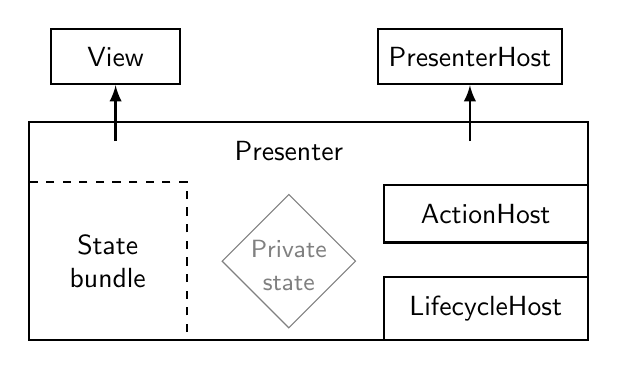
\begin{tikzpicture}[]

	\node (presenter) [align=center] at (-1.5,-0.2) {Presenter};
	
		\node (actionhost) [align=center, text width=6em] at (1,-1) {ActionHost};
		\node (actionhost-box)[thick, draw=black, fit={ (actionhost) }] {};

		\node (lifecyclehost) [align=center, text width=6em] at (1,-2.2) {LifecycleHost};
		\node (lifecyclehost-box)[thick, draw=black, fit={ (lifecyclehost) }] {};

		\node (privatestate) [color=gray!100, align=center, text width=3em] at (-1.5,-1.65) {\small Private state};
		\node (privatestate-box)[draw=gray!100, diamond, text width=3.5em] at (-1.5, -1.6) {};

		\node (statebundle) [minimum size=5em, color=black, align=center, text width=3em] at (-3.8,-1.6) {State bundle};
		\node (statebundle-box)[thick, draw=black, dashed, fit={ (statebundle) }] {};
		
	\node (presenter-box)[thick, draw=black, fit={ (presenter) (actionhost) (lifecyclehost) (privatestate) (statebundle) }] {};

	\node (view) [draw=black, thick, minimum size=2em, text width=4em, align=center] at (-3.7, 1) {View};

	\node (host) [draw=black, thick, minimum size=2em, text width=6em, align=center] at (0.8, 1) {PresenterHost};
	
	\node (view-anchor) at (-3.7, -0.2) {};
	
	\node (host-anchor) at (0.8, -0.2) {};
	
	\draw[->=triangle, line width=0.1em] (view-anchor) to (view);
	\draw[->, line width=0.1em] (host-anchor) to (host);
	
	\end{tikzpicture}

\end{document}